\subsection{\href{http://www.gruponoto.com}{Noto Group S.A.}}
   \hypertarget{subsec:noto}
   Noto Group S.A is currently developing and manufacturing electronic equipment for electromedicine
   aesthetics among which stand out:\\
      \cvlistitem{Tripolar radiofrequency.}
      \cvlistitem{Electroporador.}
      \cvlistitem{microdermabrasion.}
      \cvlistitem{Cavitator.}
      \cvlistitem{Light therapy.}
      \cvlistitem{Portable electrostimulator.}
      \cvlistitem{Medical certified power supplies.}

      The figures \ref{fig:noto1}, \ref{fig:noto2} y \ref{fig:noto3} shown some of the equipments:
   \begin{figure}
      \begin{center}
         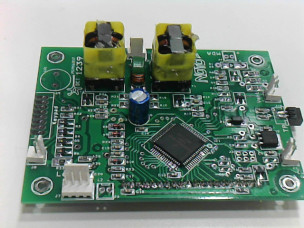
\includegraphics[width=0.24\textwidth]{portfolio/noto5.jpg}
         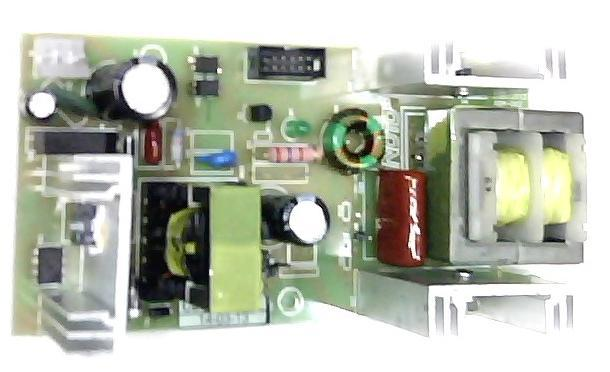
\includegraphics[width=0.24\textwidth]{portfolio/noto6.jpg}
         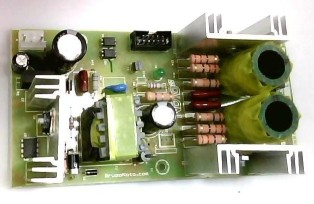
\includegraphics[width=0.24\textwidth]{portfolio/noto7.jpg}
         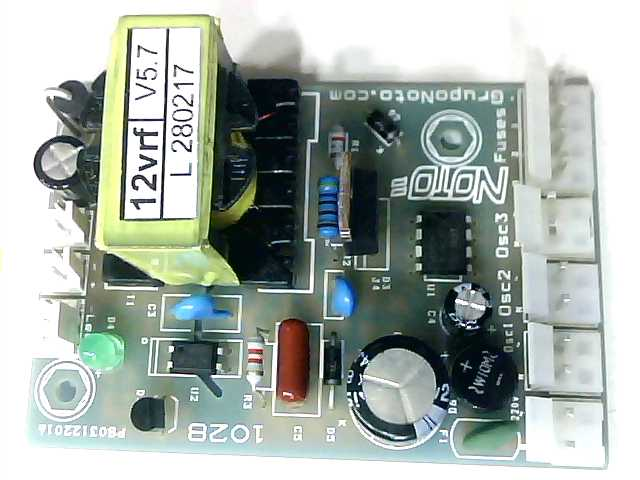
\includegraphics[width=0.24\textwidth]{portfolio/noto8.jpg}
      \end{center}
      \caption{Power equipments, power supplies, oscilatores, TH and SMD mounting styles}
      \label{fig:noto1}
   \end{figure}
   \begin{figure}
      \begin{center}
         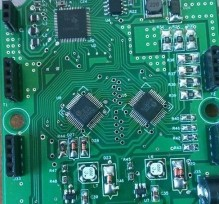
\includegraphics[width=0.24\textwidth]{portfolio/noto9.jpg}
         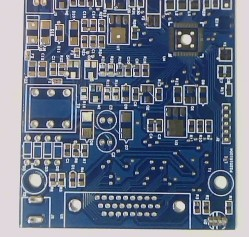
\includegraphics[width=0.24\textwidth]{portfolio/noto10.jpg}
         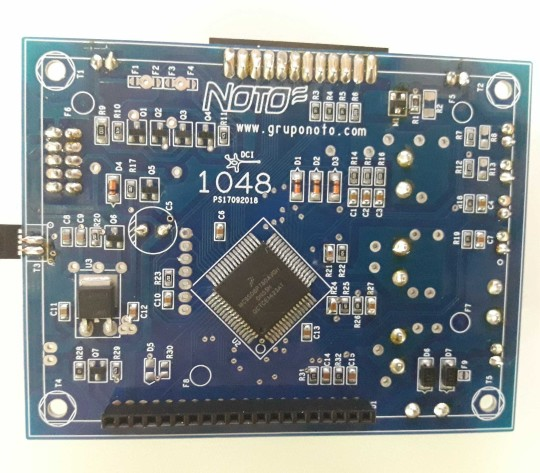
\includegraphics[width=0.24\textwidth]{portfolio/noto11.jpg}
         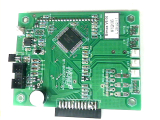
\includegraphics[width=0.24\textwidth]{portfolio/noto12.jpg}
      \end{center}
      \caption{Controlller boards, LCD controllers, PWM drivers, communications channels, signal generators, TH y SMD 1206, 0805 y 0603 techonolgies used.}
      \label{fig:noto2}
   \end{figure}
   \begin{figure}
      \begin{center}
         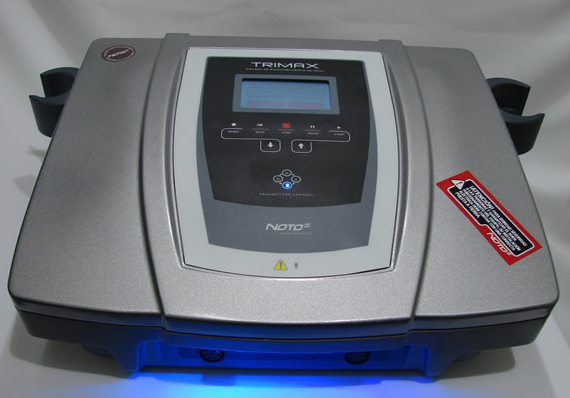
\includegraphics[width=0.24\textwidth]{portfolio/noto1.jpg}
         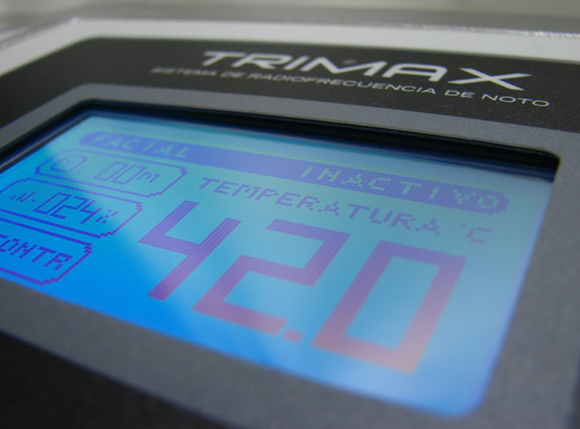
\includegraphics[width=0.24\textwidth]{portfolio/noto2.jpg}
         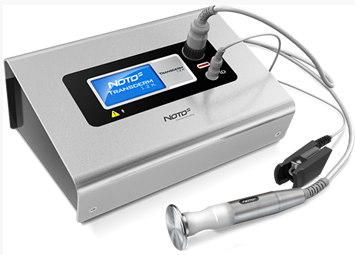
\includegraphics[width=0.24\textwidth]{portfolio/noto3.jpg}
         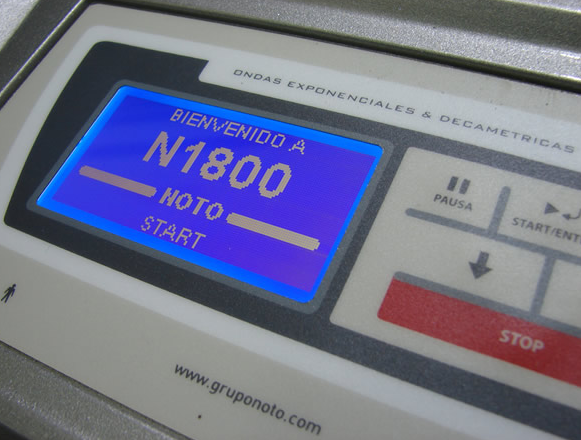
\includegraphics[width=0.24\textwidth]{portfolio/noto4.jpg}
      \end{center}
      \caption{Manugactured equipment by disenioconingenio and comercialized by Noto Group}
      \label{fig:noto3}
   \end{figure}
